% Options for packages loaded elsewhere
\PassOptionsToPackage{unicode}{hyperref}
\PassOptionsToPackage{hyphens}{url}
%
\documentclass[
]{book}
\usepackage{amsmath,amssymb}
\usepackage{lmodern}
\usepackage{ifxetex,ifluatex}
\ifnum 0\ifxetex 1\fi\ifluatex 1\fi=0 % if pdftex
  \usepackage[T1]{fontenc}
  \usepackage[utf8]{inputenc}
  \usepackage{textcomp} % provide euro and other symbols
\else % if luatex or xetex
  \usepackage{unicode-math}
  \defaultfontfeatures{Scale=MatchLowercase}
  \defaultfontfeatures[\rmfamily]{Ligatures=TeX,Scale=1}
\fi
% Use upquote if available, for straight quotes in verbatim environments
\IfFileExists{upquote.sty}{\usepackage{upquote}}{}
\IfFileExists{microtype.sty}{% use microtype if available
  \usepackage[]{microtype}
  \UseMicrotypeSet[protrusion]{basicmath} % disable protrusion for tt fonts
}{}
\makeatletter
\@ifundefined{KOMAClassName}{% if non-KOMA class
  \IfFileExists{parskip.sty}{%
    \usepackage{parskip}
  }{% else
    \setlength{\parindent}{0pt}
    \setlength{\parskip}{6pt plus 2pt minus 1pt}}
}{% if KOMA class
  \KOMAoptions{parskip=half}}
\makeatother
\usepackage{xcolor}
\IfFileExists{xurl.sty}{\usepackage{xurl}}{} % add URL line breaks if available
\IfFileExists{bookmark.sty}{\usepackage{bookmark}}{\usepackage{hyperref}}
\hypersetup{
  pdftitle={Machine Learning for Biostatistics},
  pdfauthor={Armando Teixeira-Pinto},
  hidelinks,
  pdfcreator={LaTeX via pandoc}}
\urlstyle{same} % disable monospaced font for URLs
\usepackage{color}
\usepackage{fancyvrb}
\newcommand{\VerbBar}{|}
\newcommand{\VERB}{\Verb[commandchars=\\\{\}]}
\DefineVerbatimEnvironment{Highlighting}{Verbatim}{commandchars=\\\{\}}
% Add ',fontsize=\small' for more characters per line
\usepackage{framed}
\definecolor{shadecolor}{RGB}{248,248,248}
\newenvironment{Shaded}{\begin{snugshade}}{\end{snugshade}}
\newcommand{\AlertTok}[1]{\textcolor[rgb]{0.94,0.16,0.16}{#1}}
\newcommand{\AnnotationTok}[1]{\textcolor[rgb]{0.56,0.35,0.01}{\textbf{\textit{#1}}}}
\newcommand{\AttributeTok}[1]{\textcolor[rgb]{0.77,0.63,0.00}{#1}}
\newcommand{\BaseNTok}[1]{\textcolor[rgb]{0.00,0.00,0.81}{#1}}
\newcommand{\BuiltInTok}[1]{#1}
\newcommand{\CharTok}[1]{\textcolor[rgb]{0.31,0.60,0.02}{#1}}
\newcommand{\CommentTok}[1]{\textcolor[rgb]{0.56,0.35,0.01}{\textit{#1}}}
\newcommand{\CommentVarTok}[1]{\textcolor[rgb]{0.56,0.35,0.01}{\textbf{\textit{#1}}}}
\newcommand{\ConstantTok}[1]{\textcolor[rgb]{0.00,0.00,0.00}{#1}}
\newcommand{\ControlFlowTok}[1]{\textcolor[rgb]{0.13,0.29,0.53}{\textbf{#1}}}
\newcommand{\DataTypeTok}[1]{\textcolor[rgb]{0.13,0.29,0.53}{#1}}
\newcommand{\DecValTok}[1]{\textcolor[rgb]{0.00,0.00,0.81}{#1}}
\newcommand{\DocumentationTok}[1]{\textcolor[rgb]{0.56,0.35,0.01}{\textbf{\textit{#1}}}}
\newcommand{\ErrorTok}[1]{\textcolor[rgb]{0.64,0.00,0.00}{\textbf{#1}}}
\newcommand{\ExtensionTok}[1]{#1}
\newcommand{\FloatTok}[1]{\textcolor[rgb]{0.00,0.00,0.81}{#1}}
\newcommand{\FunctionTok}[1]{\textcolor[rgb]{0.00,0.00,0.00}{#1}}
\newcommand{\ImportTok}[1]{#1}
\newcommand{\InformationTok}[1]{\textcolor[rgb]{0.56,0.35,0.01}{\textbf{\textit{#1}}}}
\newcommand{\KeywordTok}[1]{\textcolor[rgb]{0.13,0.29,0.53}{\textbf{#1}}}
\newcommand{\NormalTok}[1]{#1}
\newcommand{\OperatorTok}[1]{\textcolor[rgb]{0.81,0.36,0.00}{\textbf{#1}}}
\newcommand{\OtherTok}[1]{\textcolor[rgb]{0.56,0.35,0.01}{#1}}
\newcommand{\PreprocessorTok}[1]{\textcolor[rgb]{0.56,0.35,0.01}{\textit{#1}}}
\newcommand{\RegionMarkerTok}[1]{#1}
\newcommand{\SpecialCharTok}[1]{\textcolor[rgb]{0.00,0.00,0.00}{#1}}
\newcommand{\SpecialStringTok}[1]{\textcolor[rgb]{0.31,0.60,0.02}{#1}}
\newcommand{\StringTok}[1]{\textcolor[rgb]{0.31,0.60,0.02}{#1}}
\newcommand{\VariableTok}[1]{\textcolor[rgb]{0.00,0.00,0.00}{#1}}
\newcommand{\VerbatimStringTok}[1]{\textcolor[rgb]{0.31,0.60,0.02}{#1}}
\newcommand{\WarningTok}[1]{\textcolor[rgb]{0.56,0.35,0.01}{\textbf{\textit{#1}}}}
\usepackage{longtable,booktabs,array}
\usepackage{calc} % for calculating minipage widths
% Correct order of tables after \paragraph or \subparagraph
\usepackage{etoolbox}
\makeatletter
\patchcmd\longtable{\par}{\if@noskipsec\mbox{}\fi\par}{}{}
\makeatother
% Allow footnotes in longtable head/foot
\IfFileExists{footnotehyper.sty}{\usepackage{footnotehyper}}{\usepackage{footnote}}
\makesavenoteenv{longtable}
\usepackage{graphicx}
\makeatletter
\def\maxwidth{\ifdim\Gin@nat@width>\linewidth\linewidth\else\Gin@nat@width\fi}
\def\maxheight{\ifdim\Gin@nat@height>\textheight\textheight\else\Gin@nat@height\fi}
\makeatother
% Scale images if necessary, so that they will not overflow the page
% margins by default, and it is still possible to overwrite the defaults
% using explicit options in \includegraphics[width, height, ...]{}
\setkeys{Gin}{width=\maxwidth,height=\maxheight,keepaspectratio}
% Set default figure placement to htbp
\makeatletter
\def\fps@figure{htbp}
\makeatother
\setlength{\emergencystretch}{3em} % prevent overfull lines
\providecommand{\tightlist}{%
  \setlength{\itemsep}{0pt}\setlength{\parskip}{0pt}}
\setcounter{secnumdepth}{5}
\ifluatex
  \usepackage{selnolig}  % disable illegal ligatures
\fi
\usepackage[]{natbib}
\bibliographystyle{plainnat}

\title{Machine Learning for Biostatistics}
\usepackage{etoolbox}
\makeatletter
\providecommand{\subtitle}[1]{% add subtitle to \maketitle
  \apptocmd{\@title}{\par {\large #1 \par}}{}{}
}
\makeatother
\subtitle{Module 1}
\author{Armando Teixeira-Pinto}
\date{2021-07-18}

\begin{document}
\maketitle

{
\setcounter{tocdepth}{1}
\tableofcontents
}
\hypertarget{what-is-machine-learning}{%
\chapter*{What is machine learning?}\label{what-is-machine-learning}}
\addcontentsline{toc}{chapter}{What is machine learning?}

We came a long way since the term \emph{artificial intelligence} was first used by
John McCarthy in the 50's. We still don't have computers capable of conversations
such as Hal 9000 from the movie 2001: A space odyssey, but we can easily
identify some traces of \emph{synthetic intelligence} in many of our interactions
with electronic devices.

\begin{center}
\includegraphics[width=0.2\linewidth]{hal} \end{center}

When we ask something to \emph{Siri} or \emph{Alexa}, when we do a
search in the web, when we get recommendations for
movies or shopping, when our car ``reacts'' to the proximity of other objects,
when our spam email is filtered,
when we play chess against a computer or when we are automatically
identified in photos posted in social media, these are some simple examples of
sophisticated systems that, one way or another, interpret the environment and
take actions or make decision that maximize their chances of success.

Several examples can be also found in medical practice, such as patients'
access to healthcare (e.g., \href{https://search.proquest.com/openview/bf25c0b78beeffec5b3419ea7ffc79f9/1?pq-origsite=gscholar\&cbl=2042228}{Babylon}), cancer diagnosis (e.g, \href{https://jamanetwork.com/journals/jama/article-abstract/2665774}{PathAI}),
medical imaging (e.g., \href{https://www.hbs.edu/faculty/Pages/item.aspx?num=55060}{Zebra Medical Vision}), diagnostic
support systems
(e.g., \href{https://www.bizjournals.com/boston/news/2018/08/22/boston-childrens-website-to-feature-self.html}{Buoy Health}) and drugs' development.

\begin{center}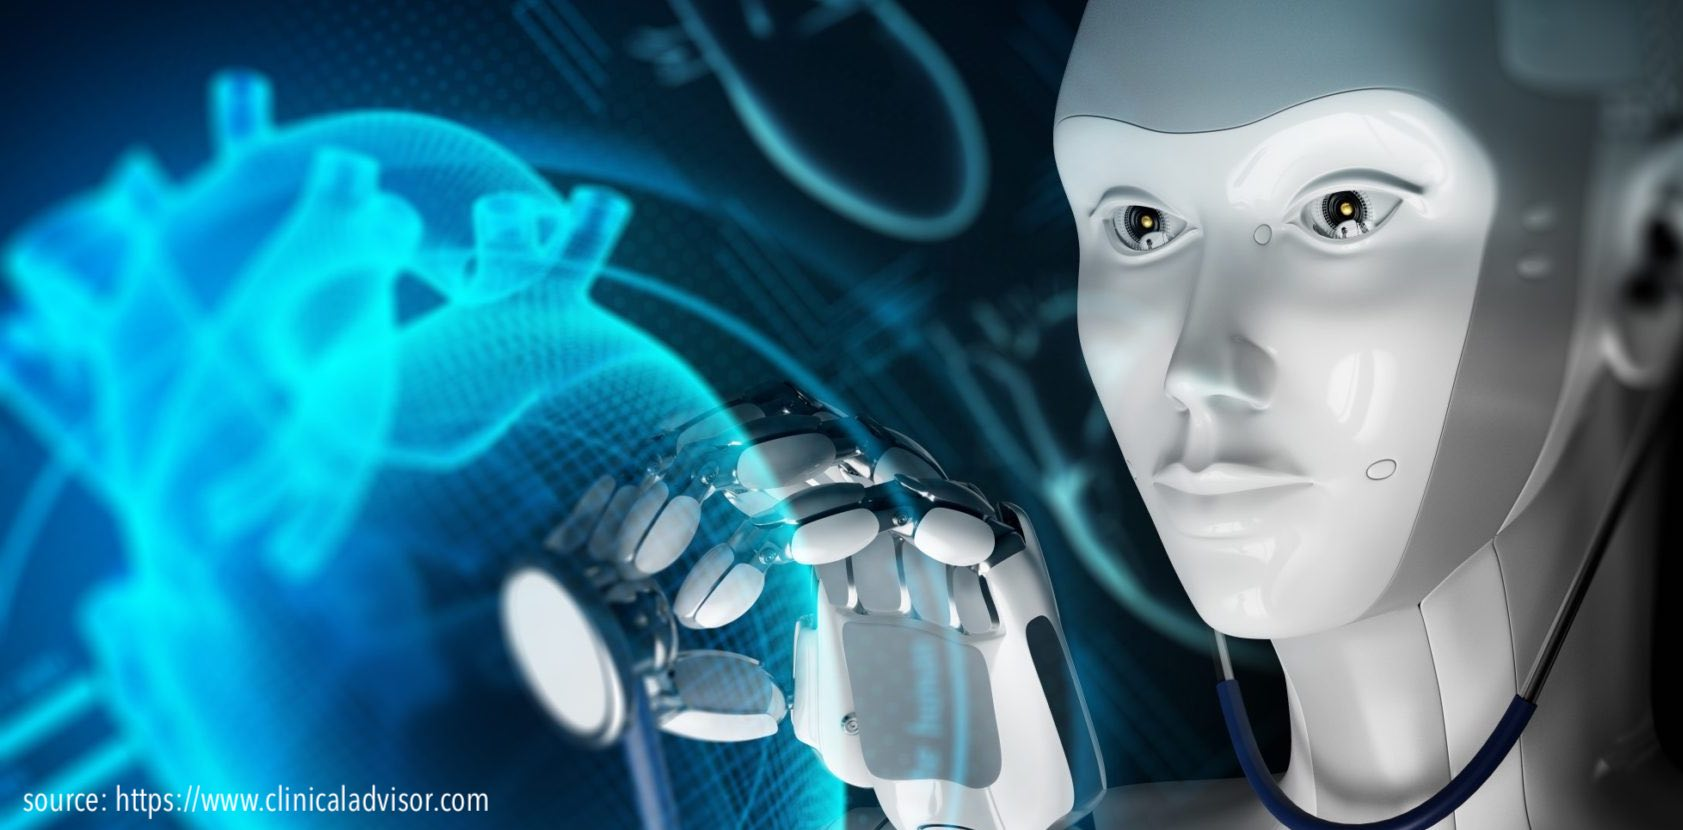
\includegraphics[width=1\linewidth]{robot} \end{center}

In parallel with the development and dissemination of AI, we have also witness a
a true data revolution in the past 30 years and a paradigm shift. Data used to
be limited and ``expensive'' to acquire, whereas nowadays we produce more data than
we can process. Many of our daily actions are stored in different databases
around the world.

This is of particular relevance because AI systems, similar to the way our
brain works, rely on two principles to ``learn'': deduction and induction (I
could also include abduction but trying to maintain things simple). Initial
AI systems relied heavily in deductive methods. The system was given (taught)
several rules and based on these rules and logic principles the
system could act. A complementary approach is to ``learn''
by recognising patterns in the data fed to the system.

\begin{center}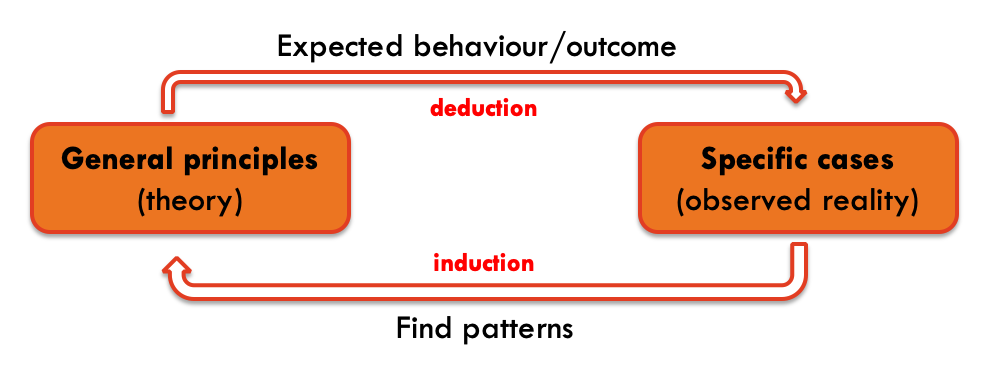
\includegraphics[width=1\linewidth]{induction} \end{center}

The challenges brought by new problems and the availability of data in
different format (image, video, text, \ldots) required new approaches outside of
the traditional statistical methods. Scientists with computer science and
engineering background, as well as statisticians, tackled these problems and
developed new methods and algorithms that take advantage of both large amounts
of data, and computational power. Despite the clear overlap with statistics,
the rapid development of this area, the major contribution from
non-statisticians to these methods, and the specificity of some of the problems,
fostered the creation of an independent scientific subject: \textbf{Machine Learning}.
Coming from statistical background (and
maybe with narrower focus) we could also call it \textbf{Statistical Learning}. In
fact, you may notice that the latter is used in the book we will follow.

\begin{center}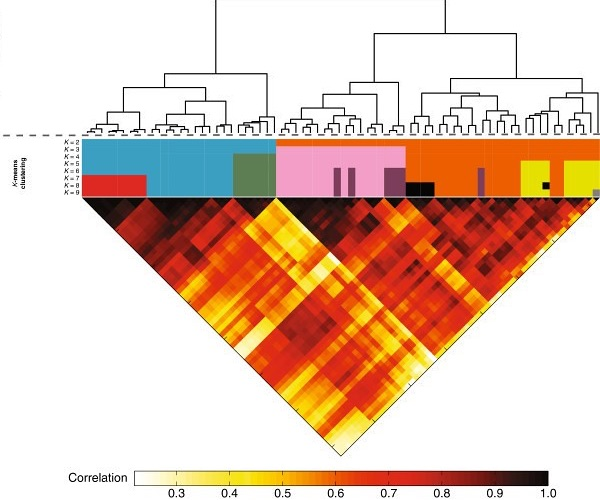
\includegraphics[width=1\linewidth]{pattern} \end{center}

An interesting perspective about \href{https://towardsdatascience.com/the-actual-difference-between-statistics-and-machine-learning-64b49f07ea3}{Machine Learning vs Statistics is presented
by M. Stewart}.

\hypertarget{datasets-used-in-the-examples}{%
\section*{Datasets used in the examples}\label{datasets-used-in-the-examples}}
\addcontentsline{toc}{section}{Datasets used in the examples}

The file \href{https://www.dropbox.com/s/7wjsfdaf0wt2kg2/bmd.csv?dl=1}{bmd.csv}
contains 169 records of bone densitometries (measurement of
bone mineral density). The following variables were collected:

\begin{itemize}
\tightlist
\item
  id -- patient's number\\
\item
  age -- patient's age
\item
  fracture -- hip fracture (fracture / no fracture)
\item
  weight\_kg -- weight measured in Kg
\item
  height\_cm -- height measure in cm\\
\item
  waiting\_time -- time the patient had to wait for the densitometry (in minutes)
\item
  bmd -- bone mineral density measure in the hip
\end{itemize}

\hypertarget{supervised-and-unsupervised-learning}{%
\chapter{Supervised and unsupervised learning}\label{supervised-and-unsupervised-learning}}

\hypertarget{introduction}{%
\section{Introduction}\label{introduction}}

The methods in \textbf{machine learning} can be broadly divided into \textbf{supervised} and
\textbf{unsupervised} learning methods.

In \textbf{supervised learning}, we have an outcome variable \(Y\) (also called output,
response, dependent variable) and a set of predictors \(\mathbf{X}\) (also called
features, dependent variables, covariates). The objective is to estimate
the function \(f(\mathbf{X})\) that connects \(Y\) and \(\mathbf{X}\). For example,

\[
Y = f(\mathbf{X}) + \varepsilon
\]

(if \(Y\) is categorical we generally consider the association of \(\mathbf{X}\) and
the \(Pr(Y=k)\))

Having a dataset with observations of \(Y\) and \(X\) (called training set), we can
use these data to find an estimate \(\hat f(\mathbf{X})\) according to some
optimisation principle.

If we specify a functional for \(f(\mathbf{X})\), such as the linear regression
model:\(f(\mathbf{X}) = \beta_0 + \beta_1X_1 + ... + \beta_p X_p\), we say that
we are using a \emph{parametric} method. If instead we allow the data to estimate
the functional form of \(f(\mathbf{X})\), such as k-nearest neighbourhood
regression, we call the method \emph{non-parametric}.

In \textbf{unsupervised learning} , the goal is to model the
underlying structure or distribution in the data without having the outcome \(Y\).
In other words, we want to analyse how the features \(\mathbf{X}\) are \emph{clustered}
or \emph{associated}. Examples of these methods are \emph{principle components analysis}
and \emph{k-means clustering}.

\hypertarget{readings}{%
\section{Readings}\label{readings}}

Read the following chapters of \emph{An introduction to statistical learning}:

\begin{itemize}
\tightlist
\item
  2.1 \href{http://faculty.marshall.usc.edu/gareth-james/ISL/ISLR\%20Seventh\%20Printing.pdf\#page=28}{What is statistical learning}
\end{itemize}

If you are using R for the first time, I encourage you to complete the section

\begin{itemize}
\tightlist
\item
  2.3 \href{http://faculty.marshall.usc.edu/gareth-james/ISL/ISLR\%20Seventh\%20Printing.pdf\#page=5}{Introduction to R}
\end{itemize}

\hypertarget{r-review}{%
\section{R review}\label{r-review}}

\hypertarget{task-1---read-a-dataset-and-create-a-new-variable}{%
\subsection*{Task 1 - Read a dataset and create a new variable}\label{task-1---read-a-dataset-and-create-a-new-variable}}
\addcontentsline{toc}{subsection}{Task 1 - Read a dataset and create a new variable}

Read the \href{https://www.dropbox.com/s/7wjsfdaf0wt2kg2/bmd.csv?dl=1}{bmd.csv}
dataset in R. You can download and read the data or use the path \emph{\url{https://www.dropbox.com/s/7wjsfdaf0wt2kg2/bmd.csv?dl=1}}

\begin{Shaded}
\begin{Highlighting}[]
\NormalTok{bmd.data }\OtherTok{\textless{}{-}} \FunctionTok{read.csv}\NormalTok{(}\StringTok{"https://www.dropbox.com/s/7wjsfdaf0wt2kg2/bmd.csv?dl=1"}\NormalTok{)}
\end{Highlighting}
\end{Shaded}

If you have downloaded the file, you need to substitute the \emph{url} above by
the path to file in your computer, e.g., ``c:\textbackslash my files\textbackslash bmd.csv''

The variable \textbf{id} is the identification of the subjects in the dataset, and
the variable \textbf{age} is their age. What is the age of the subject id=197?

\texttt{bmd.data\$age} is the vector with the ages of all the subjects. Within that
vector we need to find the one where \texttt{bmd.data\$id\ ==\ 197}. Notice that double
equal sign ``=='' is a logic statement.

If we write \texttt{bmd.data\$id\ =\ 197} we are
assigning the value 197 to the variable \textbf{id} and every subject in the dataset
gets a new value 197 for that variable.

\begin{Shaded}
\begin{Highlighting}[]
\NormalTok{bmd.data}\SpecialCharTok{$}\NormalTok{age[bmd.data}\SpecialCharTok{$}\NormalTok{id }\SpecialCharTok{==} \DecValTok{197}\NormalTok{]}
\end{Highlighting}
\end{Shaded}

\begin{verbatim}
## [1] 69.72845
\end{verbatim}

\begin{Shaded}
\begin{Highlighting}[]
\CommentTok{\#or equivalent}
\NormalTok{bmd.data[bmd.data}\SpecialCharTok{$}\NormalTok{id }\SpecialCharTok{==} \DecValTok{197}\NormalTok{, }\StringTok{"age"}\NormalTok{]}
\end{Highlighting}
\end{Shaded}

\begin{verbatim}
## [1] 69.72845
\end{verbatim}

\begin{Shaded}
\begin{Highlighting}[]
\CommentTok{\#or }
\NormalTok{bmd.data[bmd.data}\SpecialCharTok{$}\NormalTok{id }\SpecialCharTok{==} \DecValTok{197}\NormalTok{, }\DecValTok{2}\NormalTok{]  }\CommentTok{\#age is the second variable}
\end{Highlighting}
\end{Shaded}

\begin{verbatim}
## [1] 69.72845
\end{verbatim}

Let's now create a new variable \textbf{age.months} which is age in months (the
original is in years).

\begin{Shaded}
\begin{Highlighting}[]
\CommentTok{\# we just need to multiply the original by 12}
\NormalTok{bmd.data}\SpecialCharTok{$}\NormalTok{age.months }\OtherTok{\textless{}{-}}\NormalTok{ bmd.data}\SpecialCharTok{$}\NormalTok{age }\SpecialCharTok{*} \DecValTok{12}

\CommentTok{\# we can use = instead of \textless{}{-} }
\NormalTok{bmd.data}\SpecialCharTok{$}\NormalTok{age.months }\OtherTok{=}\NormalTok{ bmd.data}\SpecialCharTok{$}\NormalTok{age }\SpecialCharTok{*} \DecValTok{12}
\end{Highlighting}
\end{Shaded}

Finally, let's recode the variable \textbf{age} into age categories \textless=50, (50,60{]},
(60,70{]} and \textgreater60.

\begin{Shaded}
\begin{Highlighting}[]
\CommentTok{\# we can use the function cut() to }
\CommentTok{\#create the categories}
\NormalTok{bmd.data}\SpecialCharTok{$}\NormalTok{age.cat }\OtherTok{\textless{}{-}} \FunctionTok{cut}\NormalTok{(bmd.data}\SpecialCharTok{$}\NormalTok{age, }
                        \FunctionTok{c}\NormalTok{(}\DecValTok{0}\NormalTok{,}\DecValTok{50}\NormalTok{,}\DecValTok{60}\NormalTok{,}\DecValTok{70}\NormalTok{, }\DecValTok{100}\NormalTok{))}

\CommentTok{\# alternative }
\NormalTok{bmd.data}\SpecialCharTok{$}\NormalTok{age.cat2[bmd.data}\SpecialCharTok{$}\NormalTok{age}\SpecialCharTok{\textless{}}\DecValTok{50}\NormalTok{]                    }\OtherTok{\textless{}{-}} \DecValTok{1}
\NormalTok{bmd.data}\SpecialCharTok{$}\NormalTok{age.cat2[bmd.data}\SpecialCharTok{$}\NormalTok{age}\SpecialCharTok{\textgreater{}=}\DecValTok{50} \SpecialCharTok{\&}\NormalTok{ bmd.data}\SpecialCharTok{$}\NormalTok{age}\SpecialCharTok{\textless{}}\DecValTok{60}\NormalTok{] }\OtherTok{\textless{}{-}} \DecValTok{2}
\NormalTok{bmd.data}\SpecialCharTok{$}\NormalTok{age.cat2[bmd.data}\SpecialCharTok{$}\NormalTok{age}\SpecialCharTok{\textgreater{}=}\DecValTok{60} \SpecialCharTok{\&}\NormalTok{ bmd.data}\SpecialCharTok{$}\NormalTok{age}\SpecialCharTok{\textless{}}\DecValTok{70}\NormalTok{] }\OtherTok{\textless{}{-}} \DecValTok{3}
\NormalTok{bmd.data}\SpecialCharTok{$}\NormalTok{age.cat2[bmd.data}\SpecialCharTok{$}\NormalTok{age}\SpecialCharTok{\textgreater{}=}\DecValTok{70}\NormalTok{]                   }\OtherTok{\textless{}{-}} \DecValTok{4}

\CommentTok{\#frequencies of the categories}
\FunctionTok{table}\NormalTok{(bmd.data}\SpecialCharTok{$}\NormalTok{age.cat)}
\end{Highlighting}
\end{Shaded}

\begin{verbatim}
## 
##   (0,50]  (50,60]  (60,70] (70,100] 
##       24       45       48       52
\end{verbatim}

\textbf{TRY IT YOURSELF:}

\begin{enumerate}
\def\labelenumi{\arabic{enumi})}
\tightlist
\item
  Get the ages for all the male subjects, i.e., \texttt{bmd.data\$sex\ ==\ "M"}.
\end{enumerate}

See the solution code

\begin{Shaded}
\begin{Highlighting}[]
\NormalTok{bmd.data}\SpecialCharTok{$}\NormalTok{age[bmd.data}\SpecialCharTok{$}\NormalTok{sex }\SpecialCharTok{==} \StringTok{"M"}\NormalTok{]  }
\end{Highlighting}
\end{Shaded}

\begin{enumerate}
\def\labelenumi{\arabic{enumi})}
\setcounter{enumi}{1}
\tightlist
\item
  What is the length of the vector above? Or, in other words, how many subjects
  are male?
\end{enumerate}

See the solution code

\begin{Shaded}
\begin{Highlighting}[]
\FunctionTok{length}\NormalTok{(bmd.data}\SpecialCharTok{$}\NormalTok{age[bmd.data}\SpecialCharTok{$}\NormalTok{sex }\SpecialCharTok{==} \StringTok{"M"}\NormalTok{])}

\CommentTok{\#or}
\FunctionTok{table}\NormalTok{(bmd.data}\SpecialCharTok{$}\NormalTok{sex)}
\end{Highlighting}
\end{Shaded}

\begin{enumerate}
\def\labelenumi{\arabic{enumi})}
\setcounter{enumi}{2}
\tightlist
\item
  Using the variables \textbf{weight\_kg} and \textbf{height\_cm}, compute the body mass
  index?
  \(\frac{\text{weight in Kg}}{(\text{heigh in m})^2}\)
\end{enumerate}

See the solution code

\begin{Shaded}
\begin{Highlighting}[]
\NormalTok{bmd.data}\SpecialCharTok{$}\NormalTok{bmi }\OtherTok{\textless{}{-}}\NormalTok{ bmd.data}\SpecialCharTok{$}\NormalTok{weight\_kg }\SpecialCharTok{/}\NormalTok{(bmd.data}\SpecialCharTok{$}\NormalTok{height\_cm}\SpecialCharTok{/}\DecValTok{100}\NormalTok{)}\SpecialCharTok{**}\DecValTok{2}
\end{Highlighting}
\end{Shaded}

\hypertarget{task-2---histogram}{%
\subsection*{Task 2 - Histogram}\label{task-2---histogram}}
\addcontentsline{toc}{subsection}{Task 2 - Histogram}

There are several packages specific to graphs
\texttt{ggplot2}, \texttt{lattice}, \texttt{plotly}, \texttt{highcharter}, \texttt{sunburstR}, \texttt{dygraphs}, \texttt{rgl},\ldots{}
The \href{https://www.r-graph-gallery.com/index.html}{R Graph Gallery} is an excellent
learning resource for complex plots and visualisation

We will start with basic functions. Let's produce the histogram of the variable
\textbf{bmi} created in task 1

\begin{Shaded}
\begin{Highlighting}[]
\FunctionTok{hist}\NormalTok{(bmd.data}\SpecialCharTok{$}\NormalTok{bmi)}
\end{Highlighting}
\end{Shaded}

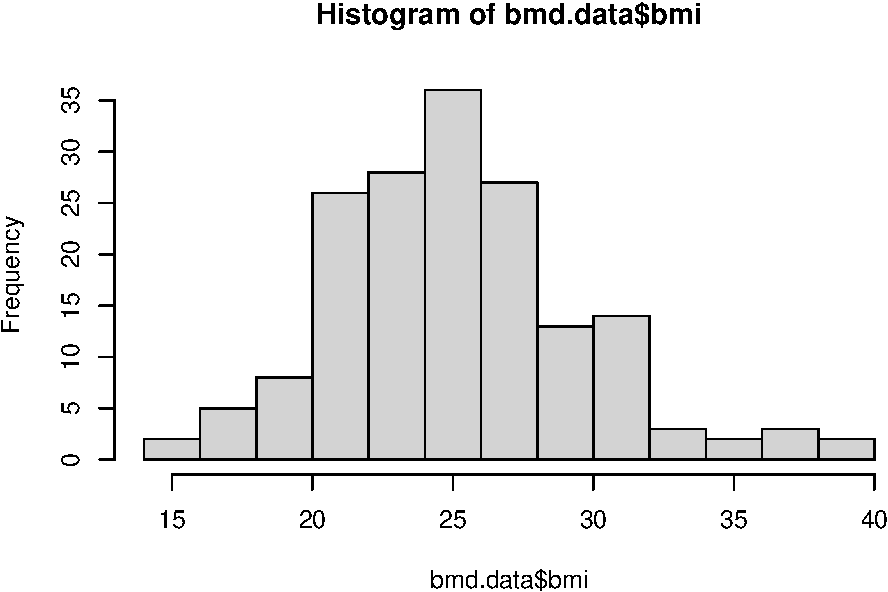
\includegraphics{_main_files/figure-latex/hisbmi -1.pdf}

Let's edit the title and x-axis label

\begin{Shaded}
\begin{Highlighting}[]
    \FunctionTok{hist}\NormalTok{(bmd.data}\SpecialCharTok{$}\NormalTok{bmi, }
         \AttributeTok{main =} \StringTok{"My 1st histogram"}\NormalTok{,     }
         \AttributeTok{xlab =} \StringTok{"Body Mass Index"}\NormalTok{)}
\end{Highlighting}
\end{Shaded}

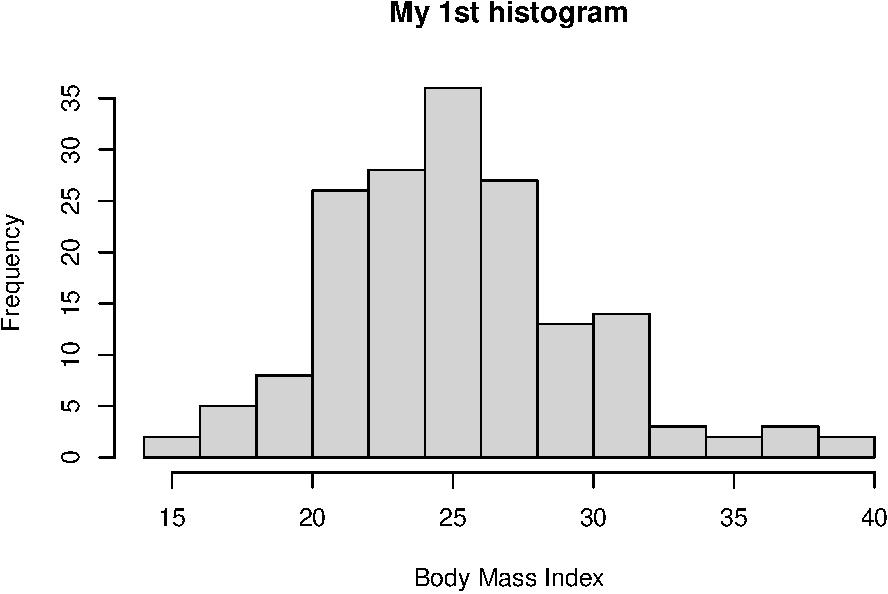
\includegraphics{_main_files/figure-latex/hisbmi2 -1.pdf}

And we can also plot the distribution for males and females, separately

\begin{Shaded}
\begin{Highlighting}[]
\CommentTok{\#histogram for males}
\FunctionTok{hist}\NormalTok{(bmd.data}\SpecialCharTok{$}\NormalTok{bmi[bmd.data}\SpecialCharTok{$}\NormalTok{sex}\SpecialCharTok{==}\StringTok{"M"}\NormalTok{ ],}
     \AttributeTok{breaks =} \DecValTok{10}\NormalTok{,                  }\CommentTok{\# number of cutoff for the bars}
     \AttributeTok{main=} \StringTok{"My 1st histogram"}\NormalTok{,  }
     \AttributeTok{xlab=} \StringTok{"Body Mass Index"}\NormalTok{,}
     \AttributeTok{col=}\FunctionTok{rgb}\NormalTok{(}\DecValTok{0}\NormalTok{,}\DecValTok{0}\NormalTok{,}\DecValTok{1}\NormalTok{,.}\DecValTok{5}\NormalTok{))           }\CommentTok{\# color of the bars}

\CommentTok{\#histogram for females}
\FunctionTok{hist}\NormalTok{(bmd.data}\SpecialCharTok{$}\NormalTok{bmi[bmd.data}\SpecialCharTok{$}\NormalTok{sex}\SpecialCharTok{==}\StringTok{"F"}\NormalTok{ ],}
      \AttributeTok{breaks =} \DecValTok{10}\NormalTok{,}
     \AttributeTok{main=} \StringTok{"My 1st histogram"}\NormalTok{,}
     \AttributeTok{xlab=} \StringTok{"Body Mass Index"}\NormalTok{, }
     \AttributeTok{col=}\FunctionTok{rgb}\NormalTok{(}\DecValTok{1}\NormalTok{,}\DecValTok{0}\NormalTok{,}\DecValTok{0}\NormalTok{,.}\DecValTok{5}\NormalTok{),}
     \AttributeTok{add=}\NormalTok{T)                      }\CommentTok{\# superimposes the histograms}

\CommentTok{\# Add legend}
\FunctionTok{legend}\NormalTok{(}\StringTok{"topright"}\NormalTok{,  }
       \AttributeTok{legend=}\FunctionTok{c}\NormalTok{(}\StringTok{"Males"}\NormalTok{,}\StringTok{"Females"}\NormalTok{), }
       \AttributeTok{col=}\FunctionTok{c}\NormalTok{(}\FunctionTok{rgb}\NormalTok{(}\DecValTok{0}\NormalTok{,}\DecValTok{0}\NormalTok{,}\DecValTok{1}\NormalTok{,}\FloatTok{0.5}\NormalTok{),  }\FunctionTok{rgb}\NormalTok{(}\DecValTok{1}\NormalTok{,}\DecValTok{0}\NormalTok{,}\DecValTok{0}\NormalTok{,}\FloatTok{0.5}\NormalTok{)), }
       \AttributeTok{pt.cex=}\DecValTok{2}\NormalTok{, }\AttributeTok{pch=}\DecValTok{15}\NormalTok{ )}
\end{Highlighting}
\end{Shaded}

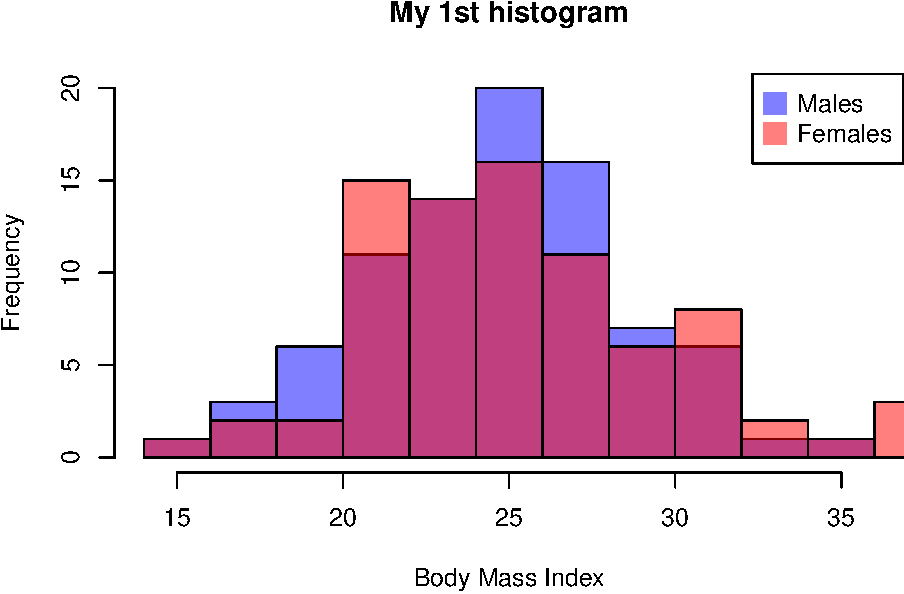
\includegraphics{_main_files/figure-latex/hisbmi3 -1.pdf}

\hypertarget{task-3---scatter-and-boxplot}{%
\subsection*{Task 3 - Scatter and boxplot}\label{task-3---scatter-and-boxplot}}
\addcontentsline{toc}{subsection}{Task 3 - Scatter and boxplot}

To see the relation between bone mineral density (\textbf{BMD}) and \textbf{age} we
can produce a scatter plot:

\begin{Shaded}
\begin{Highlighting}[]
\CommentTok{\# BMD }
\FunctionTok{plot}\NormalTok{(bmd.data}\SpecialCharTok{$}\NormalTok{age,bmd.data}\SpecialCharTok{$}\NormalTok{bmd)}
\end{Highlighting}
\end{Shaded}

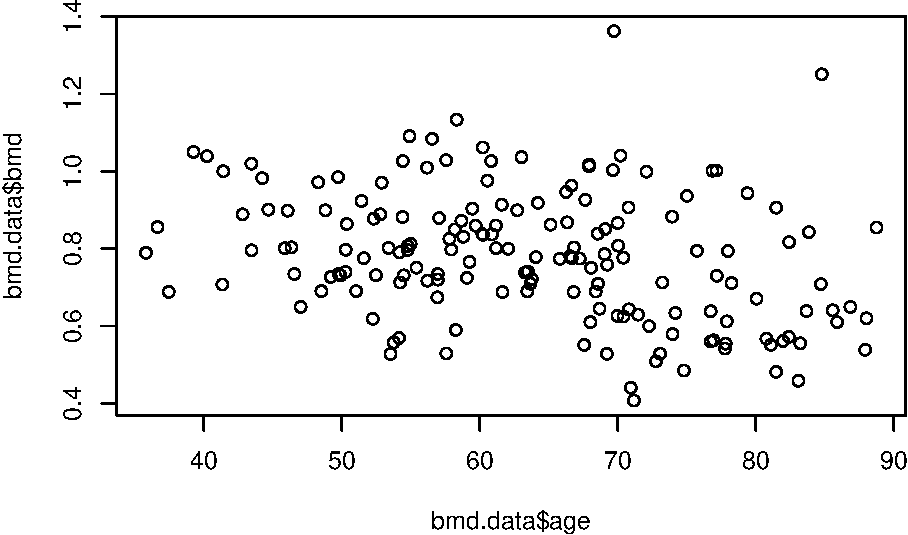
\includegraphics{_main_files/figure-latex/scatage -1.pdf}

Or a boxplot between bone mineral density (\textbf{BMD}) by categories of age created
in task 1

\begin{Shaded}
\begin{Highlighting}[]
\CommentTok{\# BMD }
\FunctionTok{boxplot}\NormalTok{(bmd.data}\SpecialCharTok{$}\NormalTok{bmd }\SpecialCharTok{\textasciitilde{}}\NormalTok{ bmd.data}\SpecialCharTok{$}\NormalTok{age.cat)}
\end{Highlighting}
\end{Shaded}

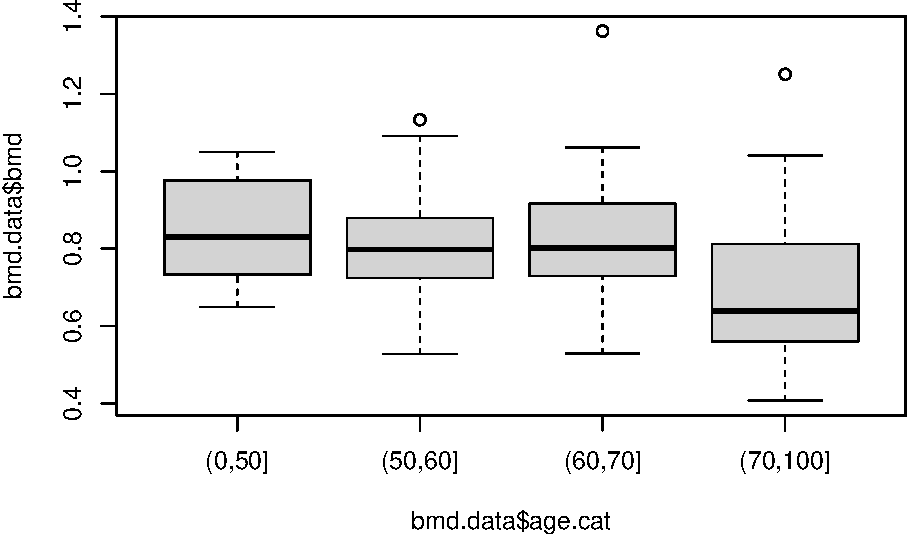
\includegraphics{_main_files/figure-latex/bpage -1.pdf}

And with a bit more work:

\begin{Shaded}
\begin{Highlighting}[]
\CommentTok{\# BMD }
\FunctionTok{boxplot}\NormalTok{(bmd.data}\SpecialCharTok{$}\NormalTok{bmd }\SpecialCharTok{\textasciitilde{}}\NormalTok{ bmd.data}\SpecialCharTok{$}\NormalTok{age.cat, }
        \AttributeTok{main =} \StringTok{"A nice boxplot (at least for a colorblind)"}\NormalTok{,}
        \AttributeTok{xlab =} \StringTok{"Age categories"}\NormalTok{,}
        \AttributeTok{ylab =} \StringTok{"Bone Mineral Density"}\NormalTok{,}
        \AttributeTok{col  =} \FunctionTok{terrain.colors}\NormalTok{(}\DecValTok{4}\NormalTok{) ) }

\CommentTok{\# Add data points}
\NormalTok{mylevels         }\OtherTok{\textless{}{-}} \FunctionTok{levels}\NormalTok{(bmd.data}\SpecialCharTok{$}\NormalTok{age.cat) }
\NormalTok{levelProportions }\OtherTok{\textless{}{-}} \FunctionTok{summary}\NormalTok{(bmd.data}\SpecialCharTok{$}\NormalTok{age.cat)}\SpecialCharTok{/}\FunctionTok{nrow}\NormalTok{(bmd.data) }

\ControlFlowTok{for}\NormalTok{(i }\ControlFlowTok{in} \DecValTok{1}\SpecialCharTok{:}\FunctionTok{length}\NormalTok{(mylevels))\{ }
\NormalTok{  thislevel  }\OtherTok{\textless{}{-}}\NormalTok{ mylevels[i] }
\NormalTok{  thisvalues }\OtherTok{\textless{}{-}}\NormalTok{ bmd.data[bmd.data}\SpecialCharTok{$}\NormalTok{age.cat }\SpecialCharTok{==}\NormalTok{ thislevel, }\StringTok{"bmd"}\NormalTok{] }
  \CommentTok{\#take the x{-}axis indices and add a jitter, }
  \CommentTok{\#proportional to the N in each level }
\NormalTok{  myjitter   }\OtherTok{\textless{}{-}} \FunctionTok{jitter}\NormalTok{(}\FunctionTok{rep}\NormalTok{(i, }\FunctionTok{length}\NormalTok{(thisvalues)),              }
                       \AttributeTok{amount=}\NormalTok{levelProportions[i]}\SpecialCharTok{/}\DecValTok{2}\NormalTok{) }
  \FunctionTok{points}\NormalTok{(myjitter, thisvalues, }
    \AttributeTok{pch=}\DecValTok{20}\NormalTok{, }\AttributeTok{col=}\FunctionTok{rgb}\NormalTok{(}\DecValTok{0}\NormalTok{,}\DecValTok{0}\NormalTok{,}\DecValTok{0}\NormalTok{,.}\DecValTok{9}\NormalTok{)) }
\NormalTok{\}}
\end{Highlighting}
\end{Shaded}

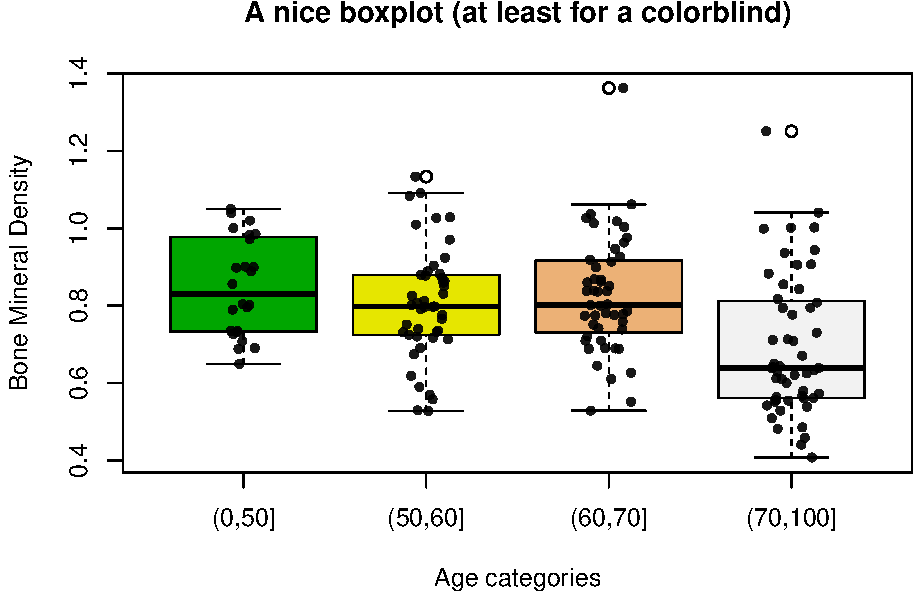
\includegraphics{_main_files/figure-latex/bpage2 -1.pdf}

\textbf{TRY IT YOURSELF:}

\begin{enumerate}
\def\labelenumi{\arabic{enumi})}
\tightlist
\item
  Plot a scatter for the relation of \textbf{bmi} and \textbf{bmd}.
\end{enumerate}

See the solution code

\begin{Shaded}
\begin{Highlighting}[]
\FunctionTok{plot}\NormalTok{(bmd.data}\SpecialCharTok{$}\NormalTok{bmi,bmd.data}\SpecialCharTok{$}\NormalTok{bmd)}
\end{Highlighting}
\end{Shaded}

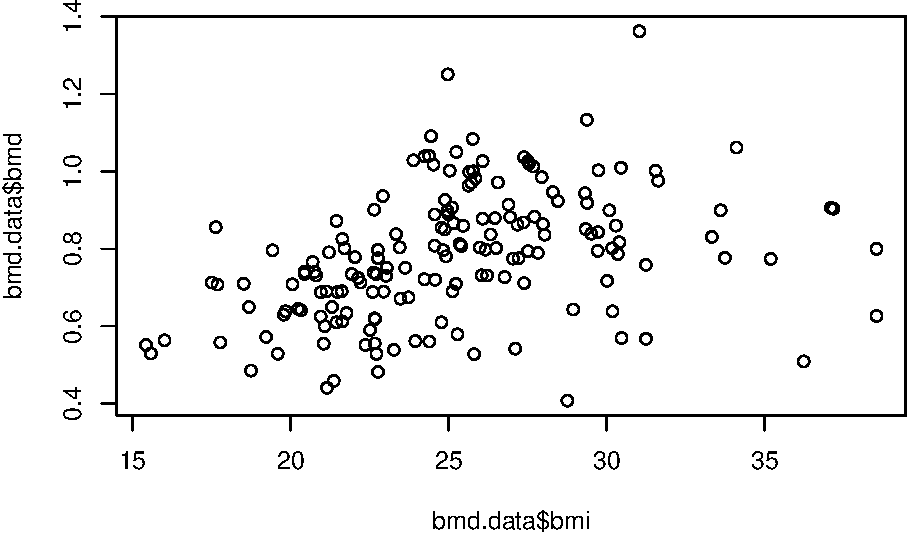
\includegraphics{_main_files/figure-latex/xx1-1.pdf}

\begin{enumerate}
\def\labelenumi{\arabic{enumi})}
\setcounter{enumi}{1}
\tightlist
\item
  Plot a scatter for the relation of \textbf{bmi} and \textbf{bmd} with the dots
  painted by the variable \textbf{sex}.
\end{enumerate}

See the solution code

\begin{Shaded}
\begin{Highlighting}[]
\FunctionTok{plot}\NormalTok{(bmd.data}\SpecialCharTok{$}\NormalTok{bmi,bmd.data}\SpecialCharTok{$}\NormalTok{bmd, }
     \AttributeTok{pch=}\DecValTok{20}\NormalTok{,}
     \AttributeTok{col=} \FunctionTok{ifelse}\NormalTok{(bmd.data}\SpecialCharTok{$}\NormalTok{sex}\SpecialCharTok{==}\StringTok{"M"}\NormalTok{,  }\CommentTok{\#blue for males}
                 \StringTok{"blue"}\NormalTok{,             }\CommentTok{\#red for females}
                 \StringTok{"red"}\NormalTok{)}
\NormalTok{     )}

\CommentTok{\# Add legend}
\FunctionTok{legend}\NormalTok{(}\StringTok{"topright"}\NormalTok{,  }
       \AttributeTok{legend=}\FunctionTok{c}\NormalTok{(}\StringTok{"Males"}\NormalTok{,}\StringTok{"Females"}\NormalTok{), }
       \AttributeTok{col=}\FunctionTok{c}\NormalTok{(}\StringTok{"blue"}\NormalTok{,  }\StringTok{"red"}\NormalTok{), }
       \AttributeTok{pt.cex=}\DecValTok{3}\NormalTok{, }\AttributeTok{pch=}\DecValTok{20}\NormalTok{ )}
\end{Highlighting}
\end{Shaded}

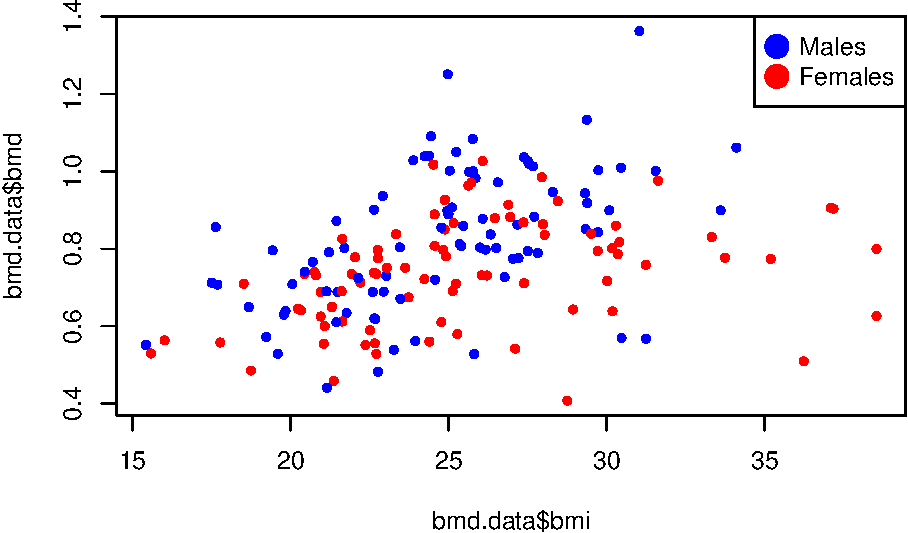
\includegraphics{_main_files/figure-latex/xx2-1.pdf}

\hypertarget{model-accuracy}{%
\chapter{Model Accuracy}\label{model-accuracy}}

\hypertarget{maccuracy.intro}{%
\section{Introduction}\label{maccuracy.intro}}

In \textbf{machine learning} there is a big emphasis in the prediction ability
of the model. We will see several measures of performance for different methods
but one commonly used measure (in particular when \(Y\) is continuous) is the
\textbf{mean squared error (MSE)}.

The MSE is defined as:

\[
MSE = E \big[ (\hat{Y} - Y)^2 \big]
\]

where \(\hat{Y} = \hat f(\mathbf{X})\).

We can estimate the MSE using the same data (training data)
that we have used to obtain
\(\hat f(\mathbf{X})\) (the training MSE). If we have \(n\) observations,

\[
y=
\begin{pmatrix}
y_1 \\
y_2 \\
\vdots\\
y_n
\end{pmatrix}
\]

and

\[
 \mathbf{x}=
\begin{pmatrix}
x_{11} & \dots & x_{p1} \\
x_{12} & \dots & x_{p2} \\
\vdots & \vdots & \vdots\\
x_{1n} & \dots & x_{pn}
\end{pmatrix}
\]

the estimate of MSE based on the data would then be:

\(MSE = \frac{1}{n} \sum_{i=1}^n \big(y_i - \hat f(x_{1i},\dots, x_{pi})\big)^2\\\)

However, this MSE tends to overestimate the true predictive ability,
given that the model is optimised to the training data. Ideally, we
would like to evaluate the performance of the model
in an independent dataset (test data) with \(y^{new}\) and \(\mathbf{x}^{new}\).

One important concept associated with the MSE that we will be talking later in
the coming modules, is the \emph{bias-variance tradeoff}. The MSE can be decomposed
into \emph{bias} and \emph{variance}:

\begin{equation}
MSE  = \mathrm{E} \big[ (\hat{Y} - Y)^2 \big] \\
 =\mathrm{E} \big(\hat{Y}^2\big) + \mathrm{E}\big(Y^2\big) - 2\mathrm{E}(\hat{Y}Y) \\  = \mathrm{E} \big(\hat{Y}^2\big) + Y^2 - 2Y\mathrm{E}(\hat{Y}) + \mathrm{E}^2(\hat{Y}) - \mathrm{E}^2(\hat{Y})\\
 =\underbrace{ \big[\mathrm{E}(\hat{Y}) - Y \big]^2}_{bias^2} + \underbrace{\mathrm{E} \big(\hat{Y}^2\big) - \mathrm{E}^2(\hat{Y})}_{var(\hat{Y})}
\end{equation}

If we use a method that produces unbiased predictions for \(Y\), such as the
ordinary least squares (OLS) for linear regression, then \(\mathrm{E}(\hat{Y}) - Y =0\).
In this case, the MSE simplifies to the \(var(\hat{Y})\).

We can see from the
decomposition, that an unbiased estimation (prediction) of \(Y\) does not lead
necessarily to the lowest MSE possible. Once again, the OLS is a good example of
this. In the case of high colinearity of the predictors \(\mathbf x\), we know that
the OLS becomes quite ``unstable'' or in other words, the OLS will have a high
variance. In this situation, it may be better to choose a different methods
that can produce some bias but will have a much lower variance, resulting in a
lower MSE. This is the case of the ridge estimator, as an alternative for the OLS when this estimator has high variance (we will talk about ridge regression in module 4).

Several methods that we will discuss use this principle of exchanging variance
for bias.

\hypertarget{maccuracy.read}{%
\section{Readings}\label{maccuracy.read}}

Read the following chapters of \emph{An introduction to statistical learning}:

\begin{itemize}
\tightlist
\item
  2.2 \href{http://faculty.marshall.usc.edu/gareth-james/ISL/ISLR\%20Seventh\%20Printing.pdf\#page=42}{Assessing Model Accuracy}
\end{itemize}

\hypertarget{R.02}{%
\section{R review}\label{R.02}}

\hypertarget{task-1---using-libraries}{%
\subsection{Task 1 - Using libraries}\label{task-1---using-libraries}}

Currently, there are more that 16,000 packages (also called libraries)
available at CRAN (Comprehensive R Archive Network). Packages are the
fundamental units of reproducible R code; they include reusable
R functions, the documentation that describes how to use them, and sample data.

We will install and use a library that produces tables similar to the ones used
for publication. This library is called tableone`.

\begin{Shaded}
\begin{Highlighting}[]
\FunctionTok{install.packages}\NormalTok{(}\StringTok{"tableone"}\NormalTok{, }
                 \AttributeTok{repos =} \StringTok{"https://cran.rstudio.com/"}\NormalTok{ ) }\CommentTok{\#downloads the package}
\end{Highlighting}
\end{Shaded}

\begin{verbatim}
## 
## The downloaded binary packages are in
##  /var/folders/nj/00dlv8r97qvczd7trdqw283w0000gn/T//RtmplFmhRc/downloaded_packages
\end{verbatim}

\begin{Shaded}
\begin{Highlighting}[]
\FunctionTok{library}\NormalTok{(tableone)            }\CommentTok{\#loads the package}
\end{Highlighting}
\end{Shaded}

Read the \href{https://www.dropbox.com/s/7wjsfdaf0wt2kg2/bmd.csv?dl=1}{bmd.csv}
dataset in R and use the function \texttt{CreateTableOne()} from the package \texttt{tableone}
to describe the variable \textbf{age}, \textbf{bmd} and \textbf{sex}.

\begin{Shaded}
\begin{Highlighting}[]
\NormalTok{bmd.data }\OtherTok{\textless{}{-}} \FunctionTok{read.csv}\NormalTok{(}\StringTok{"https://www.dropbox.com/s/7wjsfdaf0wt2kg2/bmd.csv?dl=1"}\NormalTok{)}
\FunctionTok{CreateTableOne}\NormalTok{(}\FunctionTok{c}\NormalTok{(}\StringTok{"age"}\NormalTok{, }\StringTok{"bmd"}\NormalTok{, }\StringTok{"sex"}\NormalTok{), }\AttributeTok{data=}\NormalTok{bmd.data)}
\end{Highlighting}
\end{Shaded}

\begin{verbatim}
##                  
##                   Overall      
##   n                 169        
##   age (mean (SD)) 63.63 (12.36)
##   bmd (mean (SD))  0.78 (0.17) 
##   sex = M (%)        86 (50.9)
\end{verbatim}

Let's repeat the table above but now stratified by fracture status (variable
\textbf{fracture})

\begin{Shaded}
\begin{Highlighting}[]
\FunctionTok{CreateTableOne}\NormalTok{(}\FunctionTok{c}\NormalTok{(}\StringTok{"age"}\NormalTok{, }\StringTok{"bmd"}\NormalTok{, }\StringTok{"sex"}\NormalTok{), }\AttributeTok{data=}\NormalTok{bmd.data, }\AttributeTok{strata =} \StringTok{"fracture"}\NormalTok{)}
\end{Highlighting}
\end{Shaded}

\begin{verbatim}
##                  Stratified by fracture
##                   fracture      no fracture   p      test
##   n                  50           119                    
##   age (mean (SD)) 69.77 (13.38) 61.05 (10.97) <0.001     
##   bmd (mean (SD))  0.62 (0.10)   0.85 (0.14)  <0.001     
##   sex = M (%)        25 (50.0)     61 (51.3)   1.000
\end{verbatim}

\hypertarget{task-2---using-ggplot}{%
\subsection{Task 2 - Using ggplot}\label{task-2---using-ggplot}}

\texttt{ggplot2} is a powerful library that implements a ``grammar of graphics''
developed by Wilkinson in 1999.

There are seven grammatical elements:
* Data - The dataset
* Aesthetics -How the variables in the data are mapped to visual properties
(aesthetics) of geoms
* Geometries - The visual element used for plotting the data
* Statistics - Representation of the data to help understand relationships
* Facets - Split in multiple plots
* Coordinates - Systems of coordinates
* Themes - Color schemes, font sizes,\ldots.

The combination of these elements, following certain rules, produces the plot

Suppose we want to plot the scatter for \textbf{bmd} and \textbf{age}.

First we get and load the library

\begin{Shaded}
\begin{Highlighting}[]
\FunctionTok{install.packages}\NormalTok{(}\StringTok{"ggplot2"}\NormalTok{,}
                 \AttributeTok{repos =} \StringTok{"https://cran.rstudio.com/"}\NormalTok{ )}
\end{Highlighting}
\end{Shaded}

\begin{verbatim}
## 
## The downloaded binary packages are in
##  /var/folders/nj/00dlv8r97qvczd7trdqw283w0000gn/T//RtmplFmhRc/downloaded_packages
\end{verbatim}

\begin{Shaded}
\begin{Highlighting}[]
\FunctionTok{library}\NormalTok{(ggplot2)}
\end{Highlighting}
\end{Shaded}

We start by defining the data and aesthetics

\begin{Shaded}
\begin{Highlighting}[]
\FunctionTok{ggplot}\NormalTok{(bmd.data, }\FunctionTok{aes}\NormalTok{(}\AttributeTok{x=}\NormalTok{age, }\AttributeTok{y=}\NormalTok{bmd)) }
\end{Highlighting}
\end{Shaded}

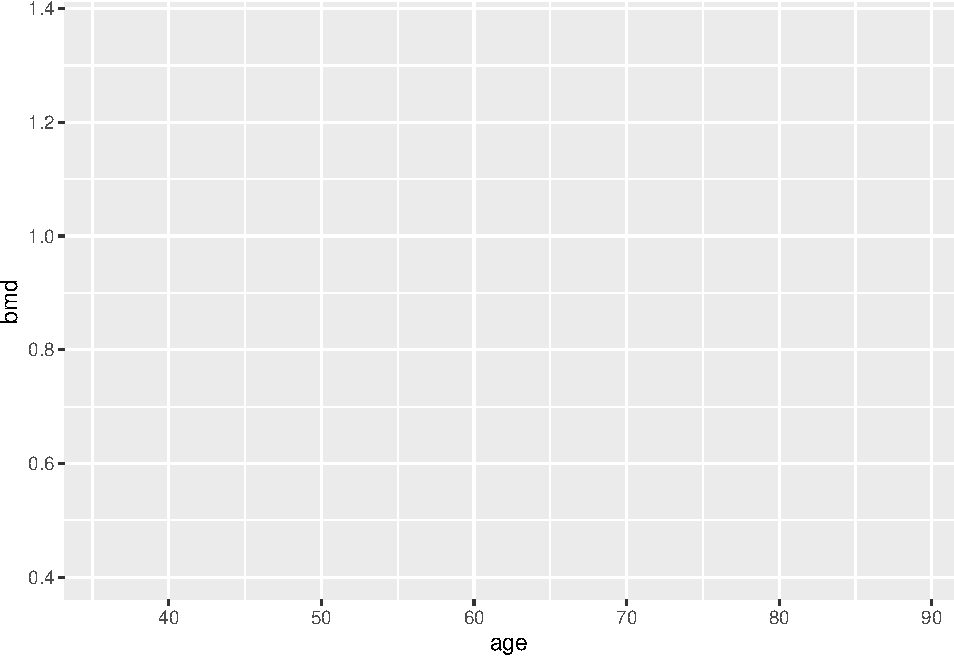
\includegraphics{_main_files/figure-latex/unnamed-chunk-12-1.pdf}

now, we add the geometry (in this case, dots)

\begin{Shaded}
\begin{Highlighting}[]
\FunctionTok{ggplot}\NormalTok{(bmd.data, }\FunctionTok{aes}\NormalTok{(}\AttributeTok{x=}\NormalTok{age, }\AttributeTok{y=}\NormalTok{bmd)) }\SpecialCharTok{+} 
        \FunctionTok{geom\_point}\NormalTok{()}
\end{Highlighting}
\end{Shaded}

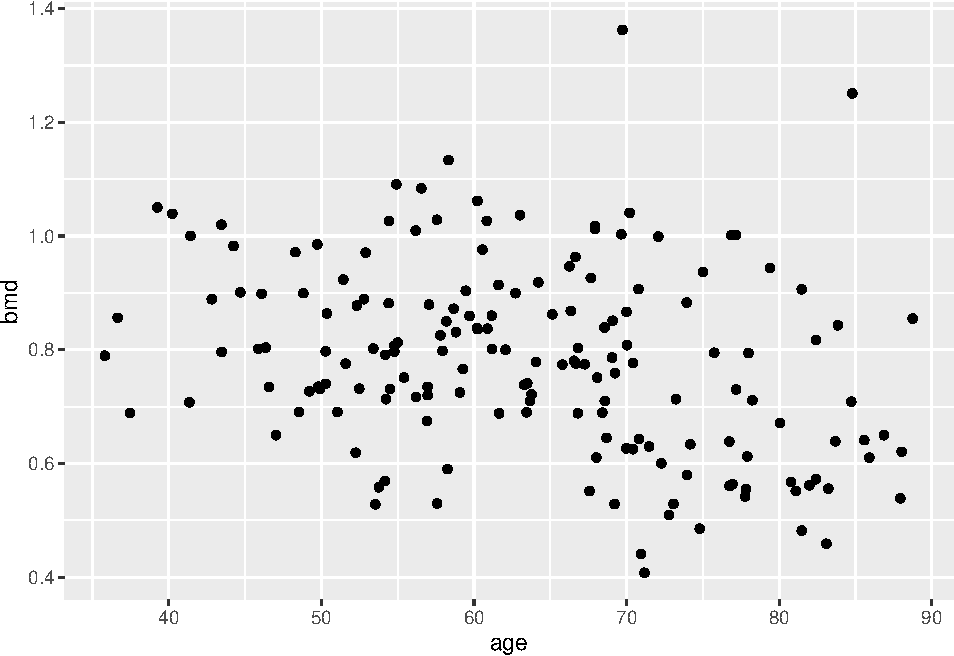
\includegraphics{_main_files/figure-latex/unnamed-chunk-13-1.pdf}

let's add a smooth line (statistics)

\begin{Shaded}
\begin{Highlighting}[]
\FunctionTok{ggplot}\NormalTok{(bmd.data, }\FunctionTok{aes}\NormalTok{(}\AttributeTok{x=}\NormalTok{age, }\AttributeTok{y=}\NormalTok{bmd)) }\SpecialCharTok{+} 
        \FunctionTok{geom\_point}\NormalTok{() }\SpecialCharTok{+} 
        \FunctionTok{stat\_smooth}\NormalTok{()  }
\end{Highlighting}
\end{Shaded}

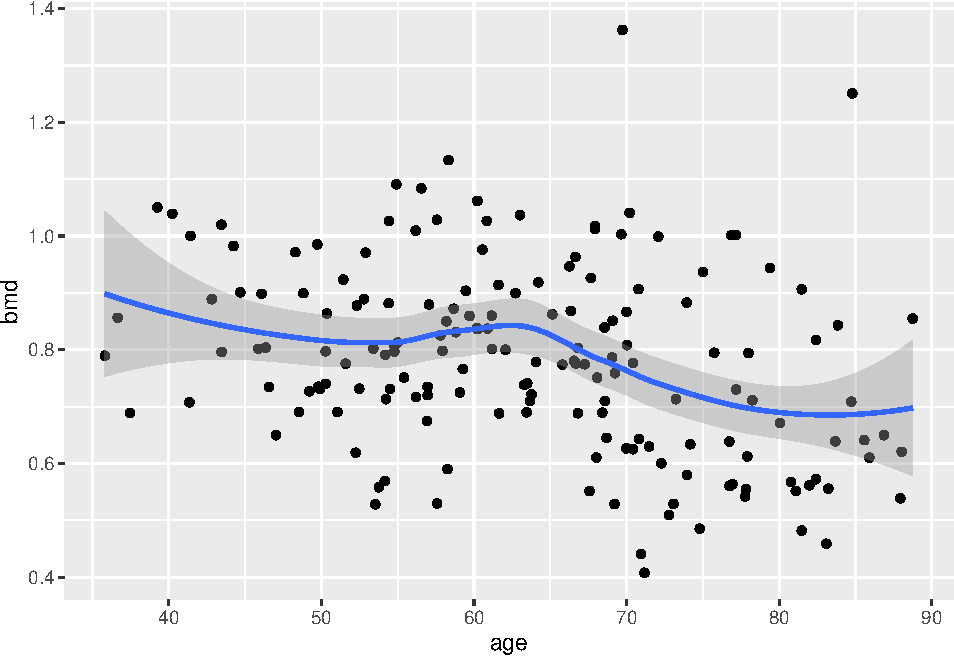
\includegraphics{_main_files/figure-latex/unnamed-chunk-14-1.pdf}

and split by sex (facets)

\begin{Shaded}
\begin{Highlighting}[]
\FunctionTok{ggplot}\NormalTok{(bmd.data, }\FunctionTok{aes}\NormalTok{(}\AttributeTok{x=}\NormalTok{age, }\AttributeTok{y=}\NormalTok{bmd)) }\SpecialCharTok{+} 
        \FunctionTok{geom\_point}\NormalTok{() }\SpecialCharTok{+} 
        \FunctionTok{stat\_smooth}\NormalTok{() }\SpecialCharTok{+} 
        \FunctionTok{facet\_grid}\NormalTok{(sex}\SpecialCharTok{\textasciitilde{}}\NormalTok{.)}
\end{Highlighting}
\end{Shaded}

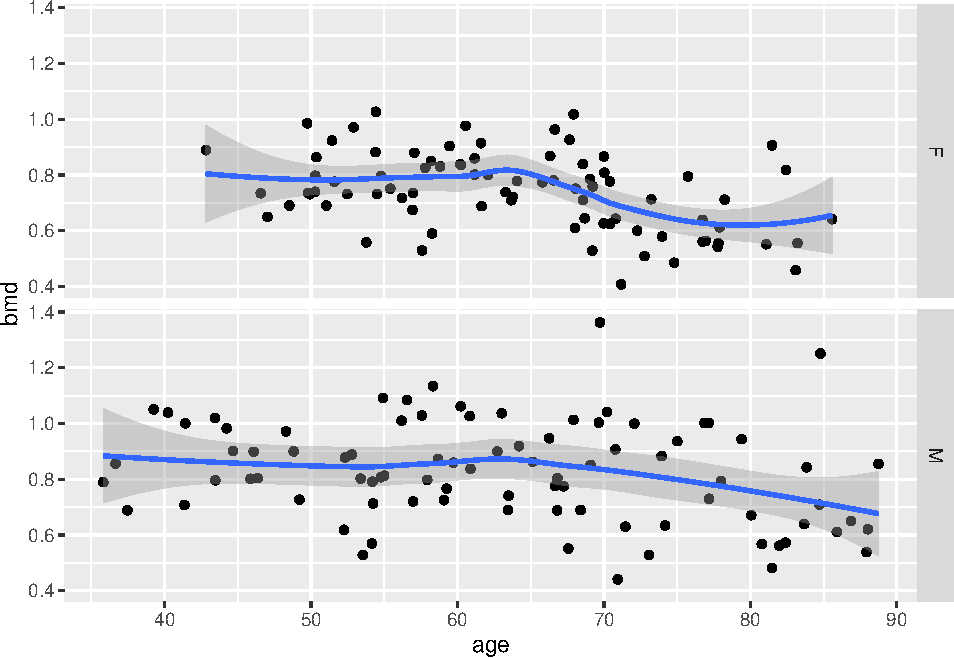
\includegraphics{_main_files/figure-latex/unnamed-chunk-15-1.pdf}

Finally, change the theme

\begin{Shaded}
\begin{Highlighting}[]
\FunctionTok{ggplot}\NormalTok{(bmd.data, }\FunctionTok{aes}\NormalTok{(}\AttributeTok{x=}\NormalTok{age, }\AttributeTok{y=}\NormalTok{bmd)) }\SpecialCharTok{+} 
        \FunctionTok{geom\_point}\NormalTok{() }\SpecialCharTok{+} 
        \FunctionTok{stat\_smooth}\NormalTok{() }\SpecialCharTok{+} 
        \FunctionTok{facet\_grid}\NormalTok{(sex}\SpecialCharTok{\textasciitilde{}}\NormalTok{.) }\SpecialCharTok{+} 
        \FunctionTok{theme\_bw}\NormalTok{()}
\end{Highlighting}
\end{Shaded}

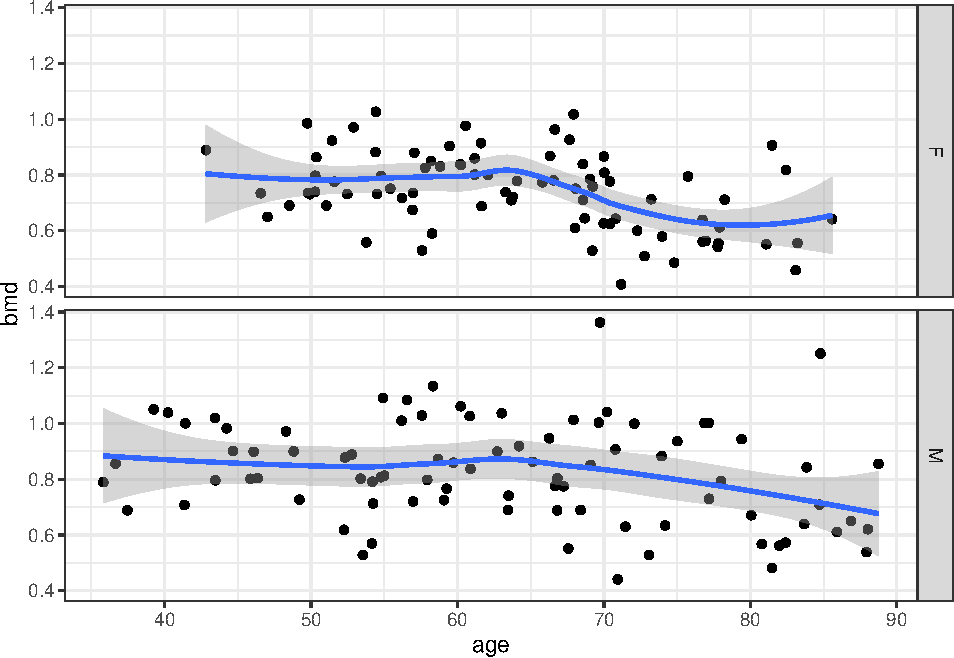
\includegraphics{_main_files/figure-latex/unnamed-chunk-16-1.pdf}

\hypertarget{task-3---writing-a-function}{%
\subsection{Task 3 - Writing a function}\label{task-3---writing-a-function}}

Write a function that computes the Body Mass Index = weight(kg)/height\(^2\)(m)
using weight and height as arguments

\begin{Shaded}
\begin{Highlighting}[]
\NormalTok{bmi.func }\OtherTok{\textless{}{-}} \ControlFlowTok{function}\NormalTok{(W, H)\{}
\NormalTok{        bmi }\OtherTok{\textless{}{-}}\NormalTok{ W}\SpecialCharTok{/}\NormalTok{H}\SpecialCharTok{\^{}}\DecValTok{2}
\NormalTok{        bmi }\OtherTok{\textless{}{-}} \FunctionTok{round}\NormalTok{(bmi,}\DecValTok{1}\NormalTok{) }\CommentTok{\#rounds 1 decimal place }
        \FunctionTok{return}\NormalTok{(}\FunctionTok{paste}\NormalTok{(}\StringTok{"The BMI is "}\NormalTok{, bmi))}
\NormalTok{\}}
\end{Highlighting}
\end{Shaded}

What is the BMI for an individual with 1.83m weighting 89Kg?

\begin{Shaded}
\begin{Highlighting}[]
\FunctionTok{bmi.func}\NormalTok{(}\DecValTok{89}\NormalTok{, }\FloatTok{1.83}\NormalTok{)}
\end{Highlighting}
\end{Shaded}

\begin{verbatim}
## [1] "The BMI is  26.6"
\end{verbatim}

\end{document}
